%% fig_mumfordgroups.tex   (generated by make_round19.py; do not edit by hand)
%% The four possible groups M^1 of the motives of a Mumford fourfold (prop:mumfordmotivic).
\documentclass[tikz,border=8pt]{standalone}
\usepackage{amsmath,amssymb}
\usetikzlibrary{arrows.meta,calc,decorations.pathreplacing}
%% palette.tex -- shared colour definitions for the figures
\definecolor{PInk}{RGB}{26,32,44}
\definecolor{PBlue}{RGB}{37,82,139}
\definecolor{PTeal}{RGB}{23,127,125}
\definecolor{POchre}{RGB}{193,138,44}
\definecolor{PClay}{RGB}{178,74,58}
\definecolor{PSlate}{RGB}{108,122,137}
\definecolor{PViolet}{RGB}{110,86,150}
\definecolor{WBlue}{RGB}{223,234,246}
\definecolor{WTeal}{RGB}{220,238,236}
\definecolor{WOchre}{RGB}{250,240,218}
\definecolor{WClay}{RGB}{247,229,224}
\definecolor{WSlate}{RGB}{238,241,244}
\definecolor{PMag}{RGB}{158,58,110}
\definecolor{PGrass}{RGB}{62,124,66}
\definecolor{PAmber}{RGB}{214,112,38}
\definecolor{PIndigo}{RGB}{58,64,140}
\definecolor{PRule}{RGB}{176,186,197}

%% shared macros so the standalone figures match the paper
\providecommand{\QQ}{\mathbb{Q}}
\providecommand{\ZZ}{\mathbb{Z}}
\providecommand{\RR}{\mathbb{R}}
\providecommand{\CC}{\mathbb{C}}
\providecommand{\PP}{\mathbb{P}}
\providecommand{\Kx}{K^{\times}}
\providecommand{\HW}{W}
\providecommand{\Nm}{\mathrm{N}}
\providecommand{\Hdg}{\mathrm{Hdg}}
\providecommand{\NS}{\mathrm{NS}}
\providecommand{\cA}{\mathcal{A}}
\providecommand{\cD}{\mathcal{D}}
\providecommand{\cF}{\mathcal{F}}
\providecommand{\cP}{\mathcal{P}}
\providecommand{\cO}{\mathcal{O}}
\providecommand{\cQ}{\mathcal{Q}}
\providecommand{\bbar}[1]{\overline{#1}}
\providecommand{\ch}{\operatorname{ch}}
\providecommand{\End}{\mathrm{End}}
\providecommand{\Ext}{\operatorname{Ext}}
\providecommand{\Supp}{\operatorname{Supp}}

\begin{document}
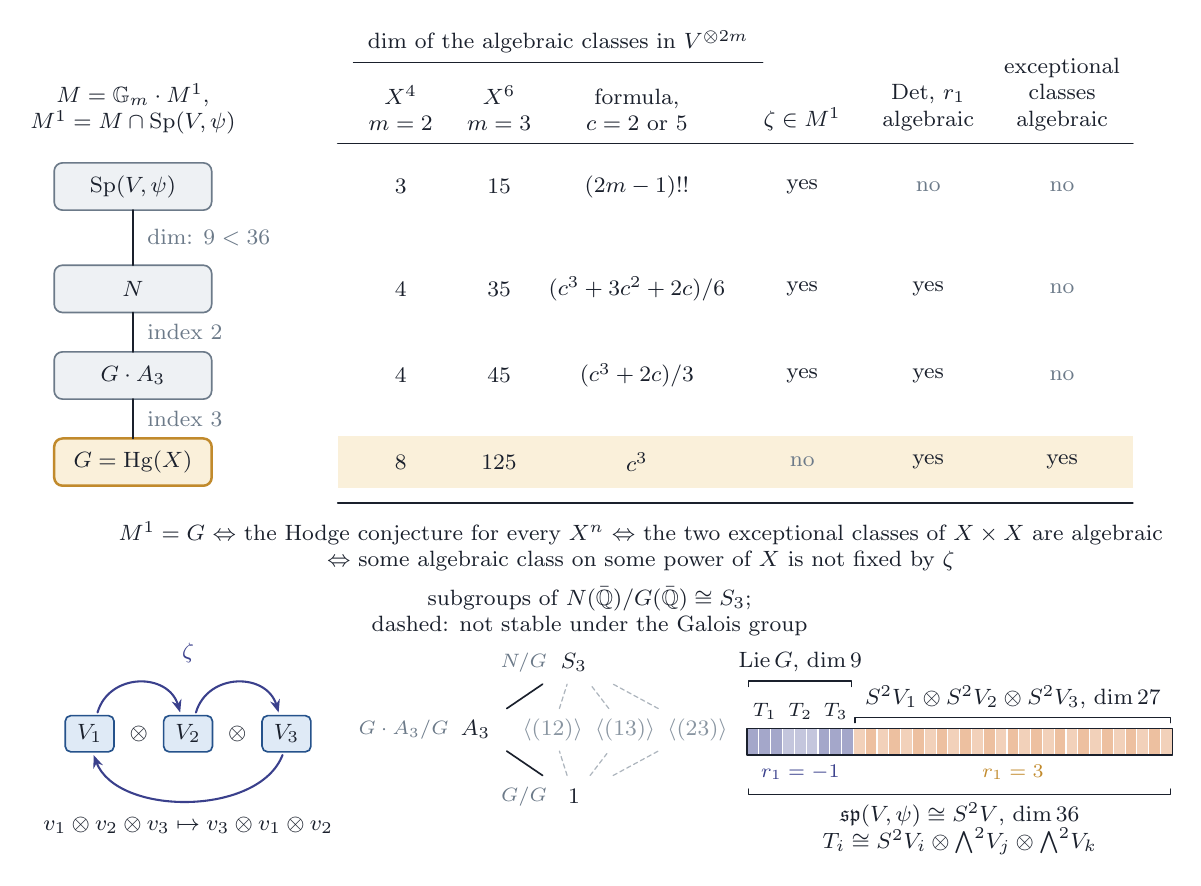
\begin{tikzpicture}[x=1cm,y=1cm,line join=round,line cap=round,
  font=\small,text=PInk,lbl/.style={inner sep=1pt}]
  \path[fill=WOchre,draw=none,rounded corners=3.0pt] (-0.0500,-0.3000) rectangle (1.9500,0.3000);
  \path[fill=WSlate,draw=none,rounded corners=3.0pt] (-0.0500,0.8000) rectangle (1.9500,1.4000);
  \path[fill=WSlate,draw=none,rounded corners=3.0pt] (-0.0500,1.9000) rectangle (1.9500,2.5000);
  \path[fill=WSlate,draw=none,rounded corners=3.0pt] (-0.0500,3.2000) rectangle (1.9500,3.8000);
  \path[fill=WOchre,draw=none] (3.5500,-0.3300) rectangle (13.6500,0.3300);
  \path[fill=WBlue,draw=none,rounded corners=2.0pt] (0.0900,-3.6800) rectangle (0.7100,-3.2200);
  \path[fill=WBlue,draw=none,rounded corners=2.0pt] (1.3400,-3.6800) rectangle (1.9600,-3.2200);
  \path[fill=WBlue,draw=none,rounded corners=2.0pt] (2.5900,-3.6800) rectangle (3.2100,-3.2200);
  \path[fill=none,draw=POchre,line width=0.90pt,rounded corners=3.0pt] (-0.0500,-0.3000) rectangle (1.9500,0.3000);
  \path[fill=none,draw=PSlate,line width=0.60pt,rounded corners=3.0pt] (-0.0500,0.8000) rectangle (1.9500,1.4000);
  \path[fill=none,draw=PSlate,line width=0.60pt,rounded corners=3.0pt] (-0.0500,1.9000) rectangle (1.9500,2.5000);
  \path[fill=none,draw=PSlate,line width=0.60pt,rounded corners=3.0pt] (-0.0500,3.2000) rectangle (1.9500,3.8000);
  \draw[PInk,line width=0.7pt] (0.9500,0.3000) -- (0.9500,0.8000);
  \draw[PInk,line width=0.7pt] (0.9500,1.4000) -- (0.9500,1.9000);
  \draw[PInk,line width=0.7pt] (0.9500,2.5000) -- (0.9500,3.2000);
  \draw[PInk,line width=0.5pt] (3.5500,4.0500) -- (13.6500,4.0500);
  \draw[PInk,line width=0.35pt] (3.7500,5.0700) -- (8.9500,5.0700);
  \draw[PInk,line width=0.5pt] (3.5500,-0.5200) -- (13.6500,-0.5200);
  \path[fill=none,draw=PBlue,line width=0.60pt,rounded corners=2.0pt] (0.0900,-3.6800) rectangle (0.7100,-3.2200);
  \path[fill=none,draw=PBlue,line width=0.60pt,rounded corners=2.0pt] (1.3400,-3.6800) rectangle (1.9600,-3.2200);
  \path[fill=none,draw=PBlue,line width=0.60pt,rounded corners=2.0pt] (2.5900,-3.6800) rectangle (3.2100,-3.2200);
  \draw[PIndigo,line width=0.75pt,-{Stealth[length=4.6pt,width=3.6pt]}] (0.5000,-3.1800) .. controls (0.6500,-2.6700) and (1.4000,-2.6700) .. (1.5500,-3.1800);
  \draw[PIndigo,line width=0.75pt,-{Stealth[length=4.6pt,width=3.6pt]}] (1.7500,-3.1800) .. controls (1.9000,-2.6700) and (2.6500,-2.6700) .. (2.8000,-3.1800);
  \draw[PIndigo,line width=0.75pt,-{Stealth[length=4.6pt,width=3.6pt]}] (2.8500,-3.7200) .. controls (2.5500,-4.5000) and (0.7500,-4.5000) .. (0.4500,-3.7200);
  \draw[PInk,line width=0.6pt] (6.1529,-3.9800) -- (5.6971,-3.6700);
  \draw[PInk,line width=0.6pt] (5.6971,-3.1300) -- (6.1529,-2.8200);
  \draw[PSlate!55,line width=0.45pt,dash pattern=on 1.6pt off 1.2pt] (6.4642,-3.9800) -- (6.3658,-3.6700);
  \draw[PSlate!55,line width=0.45pt,dash pattern=on 1.6pt off 1.2pt] (6.3658,-3.1300) -- (6.4642,-2.8200);
  \draw[PSlate!55,line width=0.45pt,dash pattern=on 1.6pt off 1.2pt] (6.7565,-3.9800) -- (6.9935,-3.6700);
  \draw[PSlate!55,line width=0.45pt,dash pattern=on 1.6pt off 1.2pt] (6.9935,-3.1300) -- (6.7565,-2.8200);
  \draw[PSlate!55,line width=0.45pt,dash pattern=on 1.6pt off 1.2pt] (7.0487,-3.9800) -- (7.6213,-3.6700);
  \draw[PSlate!55,line width=0.45pt,dash pattern=on 1.6pt off 1.2pt] (7.6213,-3.1300) -- (7.0487,-2.8200);
  \path[fill=PIndigo!46!white,draw=white,line width=0.40pt] (8.7500,-3.7200) rectangle (8.9000,-3.3800);
  \path[fill=PIndigo!46!white,draw=white,line width=0.40pt] (8.9000,-3.7200) rectangle (9.0500,-3.3800);
  \path[fill=PIndigo!46!white,draw=white,line width=0.40pt] (9.0500,-3.7200) rectangle (9.2000,-3.3800);
  \path[fill=PIndigo!30!white,draw=white,line width=0.40pt] (9.2000,-3.7200) rectangle (9.3500,-3.3800);
  \path[fill=PIndigo!30!white,draw=white,line width=0.40pt] (9.3500,-3.7200) rectangle (9.5000,-3.3800);
  \path[fill=PIndigo!30!white,draw=white,line width=0.40pt] (9.5000,-3.7200) rectangle (9.6500,-3.3800);
  \path[fill=PIndigo!46!white,draw=white,line width=0.40pt] (9.6500,-3.7200) rectangle (9.8000,-3.3800);
  \path[fill=PIndigo!46!white,draw=white,line width=0.40pt] (9.8000,-3.7200) rectangle (9.9500,-3.3800);
  \path[fill=PIndigo!46!white,draw=white,line width=0.40pt] (9.9500,-3.7200) rectangle (10.1000,-3.3800);
  \path[fill=PAmber!32!white,draw=white,line width=0.40pt] (10.1000,-3.7200) rectangle (10.2500,-3.3800);
  \path[fill=PAmber!44!white,draw=white,line width=0.40pt] (10.2500,-3.7200) rectangle (10.4000,-3.3800);
  \path[fill=PAmber!32!white,draw=white,line width=0.40pt] (10.4000,-3.7200) rectangle (10.5500,-3.3800);
  \path[fill=PAmber!44!white,draw=white,line width=0.40pt] (10.5500,-3.7200) rectangle (10.7000,-3.3800);
  \path[fill=PAmber!32!white,draw=white,line width=0.40pt] (10.7000,-3.7200) rectangle (10.8500,-3.3800);
  \path[fill=PAmber!44!white,draw=white,line width=0.40pt] (10.8500,-3.7200) rectangle (11.0000,-3.3800);
  \path[fill=PAmber!32!white,draw=white,line width=0.40pt] (11.0000,-3.7200) rectangle (11.1500,-3.3800);
  \path[fill=PAmber!44!white,draw=white,line width=0.40pt] (11.1500,-3.7200) rectangle (11.3000,-3.3800);
  \path[fill=PAmber!32!white,draw=white,line width=0.40pt] (11.3000,-3.7200) rectangle (11.4500,-3.3800);
  \path[fill=PAmber!44!white,draw=white,line width=0.40pt] (11.4500,-3.7200) rectangle (11.6000,-3.3800);
  \path[fill=PAmber!32!white,draw=white,line width=0.40pt] (11.6000,-3.7200) rectangle (11.7500,-3.3800);
  \path[fill=PAmber!44!white,draw=white,line width=0.40pt] (11.7500,-3.7200) rectangle (11.9000,-3.3800);
  \path[fill=PAmber!32!white,draw=white,line width=0.40pt] (11.9000,-3.7200) rectangle (12.0500,-3.3800);
  \path[fill=PAmber!44!white,draw=white,line width=0.40pt] (12.0500,-3.7200) rectangle (12.2000,-3.3800);
  \path[fill=PAmber!32!white,draw=white,line width=0.40pt] (12.2000,-3.7200) rectangle (12.3500,-3.3800);
  \path[fill=PAmber!44!white,draw=white,line width=0.40pt] (12.3500,-3.7200) rectangle (12.5000,-3.3800);
  \path[fill=PAmber!32!white,draw=white,line width=0.40pt] (12.5000,-3.7200) rectangle (12.6500,-3.3800);
  \path[fill=PAmber!44!white,draw=white,line width=0.40pt] (12.6500,-3.7200) rectangle (12.8000,-3.3800);
  \path[fill=PAmber!32!white,draw=white,line width=0.40pt] (12.8000,-3.7200) rectangle (12.9500,-3.3800);
  \path[fill=PAmber!44!white,draw=white,line width=0.40pt] (12.9500,-3.7200) rectangle (13.1000,-3.3800);
  \path[fill=PAmber!32!white,draw=white,line width=0.40pt] (13.1000,-3.7200) rectangle (13.2500,-3.3800);
  \path[fill=PAmber!44!white,draw=white,line width=0.40pt] (13.2500,-3.7200) rectangle (13.4000,-3.3800);
  \path[fill=PAmber!32!white,draw=white,line width=0.40pt] (13.4000,-3.7200) rectangle (13.5500,-3.3800);
  \path[fill=PAmber!44!white,draw=white,line width=0.40pt] (13.5500,-3.7200) rectangle (13.7000,-3.3800);
  \path[fill=PAmber!32!white,draw=white,line width=0.40pt] (13.7000,-3.7200) rectangle (13.8500,-3.3800);
  \path[fill=PAmber!44!white,draw=white,line width=0.40pt] (13.8500,-3.7200) rectangle (14.0000,-3.3800);
  \path[fill=PAmber!32!white,draw=white,line width=0.40pt] (14.0000,-3.7200) rectangle (14.1500,-3.3800);
  \path[fill=none,draw=PInk,line width=0.45pt] (8.7500,-3.7200) rectangle (14.1500,-3.3800);
  \draw[PInk,line width=0.4pt] (8.7700,-2.8500) -- (8.7700,-2.7800) -- (10.0800,-2.7800) -- (10.0800,-2.8500);
  \draw[PInk,line width=0.4pt] (10.1200,-3.3100) -- (10.1200,-3.2400) -- (14.1300,-3.2400) -- (14.1300,-3.3100);
  \draw[PInk,line width=0.4pt] (8.7700,-4.1500) -- (8.7700,-4.2200) -- (14.1300,-4.2200) -- (14.1300,-4.1500);
  \node[lbl,text=PInk,font=\footnotesize] at (0.9500,0.0000) {$G=\mathrm{Hg}(X)$};
  \node[lbl,text=PInk,font=\footnotesize] at (0.9500,1.1000) {$G\cdot A_{3}$};
  \node[lbl,text=PInk,font=\footnotesize] at (0.9500,2.2000) {$N$};
  \node[lbl,text=PInk,font=\footnotesize] at (0.9500,3.5000) {$\mathrm{Sp}(V,\psi)$};
  \node[lbl,anchor=west,text=PSlate,font=\footnotesize] at (1.0900,0.5500) {index $3$};
  \node[lbl,anchor=west,text=PSlate,font=\footnotesize] at (1.0900,1.6500) {index $2$};
  \node[lbl,anchor=west,text=PSlate,font=\footnotesize] at (1.0900,2.8500) {$\dim$: $9<36$};
  \node[lbl,anchor=south,text=PInk,font=\footnotesize,align=center] at (0.9500,4.1200) {$M=\mathbb{G}_{m}\cdot M^{1}$,\\$M^{1}=M\cap\mathrm{Sp}(V,\psi)$};
  \node[lbl,anchor=south,text=PInk,font=\footnotesize,align=center] at (4.3500,4.1700) {$X^{4}$\\$m=2$};
  \node[lbl,text=PInk,font=\footnotesize] at (4.3500,0.0000) {$8$};
  \node[lbl,text=PInk,font=\footnotesize] at (4.3500,1.1000) {$4$};
  \node[lbl,text=PInk,font=\footnotesize] at (4.3500,2.2000) {$4$};
  \node[lbl,text=PInk,font=\footnotesize] at (4.3500,3.5000) {$3$};
  \node[lbl,anchor=south,text=PInk,font=\footnotesize,align=center] at (5.6000,4.1700) {$X^{6}$\\$m=3$};
  \node[lbl,text=PInk,font=\footnotesize] at (5.6000,0.0000) {$125$};
  \node[lbl,text=PInk,font=\footnotesize] at (5.6000,1.1000) {$45$};
  \node[lbl,text=PInk,font=\footnotesize] at (5.6000,2.2000) {$35$};
  \node[lbl,text=PInk,font=\footnotesize] at (5.6000,3.5000) {$15$};
  \node[lbl,anchor=south,text=PInk,font=\footnotesize,align=center] at (7.3500,4.1700) {formula,\\$c=2$ or $5$};
  \node[lbl,text=PInk,font=\footnotesize] at (7.3500,0.0000) {$c^{3}$};
  \node[lbl,text=PInk,font=\footnotesize] at (7.3500,1.1000) {$(c^{3}+2c)/3$};
  \node[lbl,text=PInk,font=\footnotesize] at (7.3500,2.2000) {$(c^{3}+3c^{2}+2c)/6$};
  \node[lbl,text=PInk,font=\footnotesize] at (7.3500,3.5000) {$(2m-1)!!$};
  \node[lbl,anchor=south,text=PInk,font=\footnotesize,align=center] at (9.4500,4.1700) {$\zeta\in M^{1}$};
  \node[lbl,text=PSlate,font=\footnotesize] at (9.4500,0.0000) {no};
  \node[lbl,text=PInk,font=\footnotesize] at (9.4500,1.1000) {yes};
  \node[lbl,text=PInk,font=\footnotesize] at (9.4500,2.2000) {yes};
  \node[lbl,text=PInk,font=\footnotesize] at (9.4500,3.5000) {yes};
  \node[lbl,anchor=south,text=PInk,font=\footnotesize,align=center] at (11.0500,4.1700) {$\mathrm{Det}$, $r_{1}$\\algebraic};
  \node[lbl,text=PInk,font=\footnotesize] at (11.0500,0.0000) {yes};
  \node[lbl,text=PInk,font=\footnotesize] at (11.0500,1.1000) {yes};
  \node[lbl,text=PInk,font=\footnotesize] at (11.0500,2.2000) {yes};
  \node[lbl,text=PSlate,font=\footnotesize] at (11.0500,3.5000) {no};
  \node[lbl,anchor=south,text=PInk,font=\footnotesize,align=center] at (12.7500,4.1700) {exceptional\\classes\\algebraic};
  \node[lbl,text=PInk,font=\footnotesize] at (12.7500,0.0000) {yes};
  \node[lbl,text=PSlate,font=\footnotesize] at (12.7500,1.1000) {no};
  \node[lbl,text=PSlate,font=\footnotesize] at (12.7500,2.2000) {no};
  \node[lbl,text=PSlate,font=\footnotesize] at (12.7500,3.5000) {no};
  \node[lbl,anchor=south,text=PInk,font=\footnotesize] at (6.3500,5.1500) {$\dim$ of the algebraic classes in $V^{\otimes 2m}$};
  \node[lbl,anchor=north,text=PInk,font=\footnotesize,align=center] at (7.4000,-0.7200) {$M^{1}=G$ $\Leftrightarrow$ the Hodge conjecture for every $X^{n}$ $\Leftrightarrow$ the two exceptional classes of $X\times X$ are algebraic\\$\Leftrightarrow$ some algebraic class on some power of $X$ is not fixed by $\zeta$};
  \node[lbl,text=PInk,font=\footnotesize] at (0.4000,-3.4500) {$V_{1}$};
  \node[lbl,text=PInk,font=\footnotesize] at (1.6500,-3.4500) {$V_{2}$};
  \node[lbl,text=PInk,font=\footnotesize] at (2.9000,-3.4500) {$V_{3}$};
  \node[lbl,text=PInk,font=\footnotesize] at (1.0250,-3.4500) {$\otimes$};
  \node[lbl,text=PInk,font=\footnotesize] at (2.2750,-3.4500) {$\otimes$};
  \node[lbl,anchor=south,text=PIndigo,font=\footnotesize] at (1.6500,-2.5900) {$\zeta$};
  \node[lbl,anchor=north,text=PInk,font=\footnotesize] at (1.6500,-4.4700) {$v_{1}\otimes v_{2}\otimes v_{3}\mapsto v_{3}\otimes v_{1}\otimes v_{2}$};
  \node[lbl,text=PInk,font=\footnotesize] at (6.5500,-4.2500) {$1$};
  \node[lbl,text=PInk,font=\footnotesize] at (5.3000,-3.4000) {$A_{3}$};
  \node[lbl,text=PSlate!80,font=\footnotesize] at (6.2800,-3.4000) {$\langle(12)\rangle$};
  \node[lbl,text=PSlate!80,font=\footnotesize] at (7.2000,-3.4000) {$\langle(13)\rangle$};
  \node[lbl,text=PSlate!80,font=\footnotesize] at (8.1200,-3.4000) {$\langle(23)\rangle$};
  \node[lbl,text=PInk,font=\footnotesize] at (6.5500,-2.5500) {$S_{3}$};
  \node[lbl,anchor=south,text=PInk,font=\footnotesize,align=center] at (6.7500,-2.2500) {subgroups of $N(\bar\QQ)/G(\bar\QQ)\cong S_{3}$;\\dashed: not stable under the Galois group};
  \node[lbl,anchor=east,text=PSlate,font=\scriptsize] at (6.2500,-4.2500) {$G/G$};
  \node[lbl,anchor=east,text=PSlate,font=\scriptsize] at (5.0000,-3.4000) {$G\cdot A_{3}/G$};
  \node[lbl,anchor=east,text=PSlate,font=\scriptsize] at (6.2500,-2.5500) {$N/G$};
  \node[lbl,anchor=south,text=PInk,font=\scriptsize] at (8.9750,-3.3100) {$T_{1}$};
  \node[lbl,anchor=south,text=PInk,font=\scriptsize] at (9.4250,-3.3100) {$T_{2}$};
  \node[lbl,anchor=south,text=PInk,font=\scriptsize] at (9.8750,-3.3100) {$T_{3}$};
  \node[lbl,anchor=south,text=PInk,font=\footnotesize] at (9.4250,-2.7100) {$\operatorname{Lie}G$, $\dim 9$};
  \node[lbl,anchor=south,text=PInk,font=\footnotesize] at (12.1250,-3.1700) {$S^{2}V_{1}\otimes S^{2}V_{2}\otimes S^{2}V_{3}$, $\dim 27$};
  \node[lbl,anchor=north,text=PIndigo,font=\scriptsize] at (9.4250,-3.8000) {$r_{1}=-1$};
  \node[lbl,anchor=north,text=POchre,font=\scriptsize] at (12.1250,-3.8000) {$r_{1}=3$};
  \node[lbl,anchor=north,text=PInk,font=\footnotesize,align=center] at (11.4500,-4.2900) {$\mathfrak{sp}(V,\psi)\cong S^{2}V$, $\dim 36$\\$T_{i}\cong S^{2}V_{i}\otimes{\textstyle\bigwedge^{2}}V_{j}\otimes{\textstyle\bigwedge^{2}}V_{k}$};
\end{tikzpicture}
\end{document}
